% =============================================================================
%  TPF -- IA aplicada a la Robótica
%  Presentación didáctica de arquitectura: qué hace cada bloque, cómo se
%  conectan, y cómo lo que falta se engancha con lo que ya está.
%
%  Compilar:  pdflatex TPF_arquitectura.tex   (dos veces, por el índice)
%             o bien:  latexmk -pdf TPF_arquitectura.tex
%
%  Las figuras salen de ../scripts_auxiliares/figuras/, que genera el
%  cuaderno 01_calibracion_motores.ipynb.
% =============================================================================
\documentclass[aspectratio=169,10pt]{beamer}

\usetheme{metropolis}
\usepackage[T1]{fontenc}
\usepackage[utf8]{inputenc}
\usepackage[spanish,es-noquoting]{babel}
\usepackage{tikz}
\usetikzlibrary{positioning,arrows.meta,shapes.geometric,fit,backgrounds,calc,
                decorations.pathreplacing,patterns}
\usepackage{booktabs}
\usepackage{amsmath}
\usepackage{array}
\usepackage{xcolor}
\usepackage{graphicx}

\graphicspath{{../scripts_auxiliares/figuras/}}

% ------------------------------------------------------------------ Colores
% La misma paleta que las figuras del cuaderno de calibración: azul = rueda
% izquierda / nivel alto, naranja = rueda derecha / nivel bajo.
\definecolor{azul}{HTML}{2A78D6}
\definecolor{naranja}{HTML}{EB6834}
\definecolor{gris}{HTML}{52514E}
\definecolor{grisclaro}{HTML}{898781}
\definecolor{critico}{HTML}{D03B3B}
\definecolor{verde}{HTML}{0CA30C}
\definecolor{ambar}{HTML}{FAB219}

\setbeamercolor{frametitle}{bg=azul}
\setbeamercolor{progress bar}{fg=naranja}
\setbeamercolor{alerted text}{fg=critico}
\setbeamertemplate{frame numbering}[fraction]
\metroset{block=fill}

% Densidad: son diapositivas de referencia, con más texto del que suele entrar
% en una presentación. Bloques compactos y márgenes algo más angostos.
\setbeamerfont{block title}{size=\small}
\setbeamerfont{block body}{size=\small}
\setbeamerfont{itemize/enumerate body}{size=\small}
\setbeamerfont{itemize/enumerate subbody}{size=\footnotesize}
\setbeamersize{text margin left=6mm, text margin right=6mm}
\addtobeamertemplate{block begin}{\vspace{-0.25em}}{}
\addtobeamertemplate{block end}{}{\vspace{-0.55em}}
\addtobeamertemplate{block alerted begin}{\vspace{-0.25em}}{}
\addtobeamertemplate{block alerted end}{}{\vspace{-0.55em}}
\setlength{\parskip}{0.25em}

% ------------------------------------------------------------------ Atajos
\newcommand{\autornombre}{Federico Morán}   % <<< CAMBIAR SI HACE FALTA
\newcommand{\listo}{\textcolor{verde}{$\blacksquare$}}
\newcommand{\curso}{\textcolor{ambar}{$\blacksquare$}}
\newcommand{\pend}{\textcolor{grisclaro}{$\square$}}
\newcommand{\hacia}{$\rightarrow$}
\newcommand{\destaca}[1]{\textcolor{azul}{\textbf{#1}}}
\newcommand{\ojo}[1]{\textcolor{critico}{\textbf{#1}}}

% Encabezado uniforme de las fichas de bloque
\newcommand{\ficha}[4]{%
  {\footnotesize
  \begin{columns}[T,onlytextwidth]
    \begin{column}{0.485\textwidth}
      \begin{block}{Qué hace}#1\end{block}
      \begin{block}{Con quién habla}#3\end{block}
    \end{column}
    \begin{column}{0.485\textwidth}
      \begin{block}{Cómo lo hace}#2\end{block}
      \begin{block}{Estado}#4\end{block}
    \end{column}
  \end{columns}}}

% ------------------------------------------------------------------ Portada
\title{Robot autónomo de aproximación y evasión basado en visión}
\subtitle{Arquitectura del sistema: qué hace cada bloque y cómo se conectan}
\author{\autornombre}
\institute{TPF --- IA aplicada a la Robótica \\ Maestría en Inteligencia Artificial}
\date{Agosto de 2026}

\begin{document}

\maketitle

% =============================================================================
\begin{frame}{Para qué son estas diapositivas}
  \begin{block}{Objetivo}
    Poner en un solo lugar \destaca{qué estoy construyendo}, \destaca{por qué cada
    pieza está donde está}, y \destaca{cómo lo que falta se engancha con lo que
    ya funciona}.
  \end{block}

  \vspace{0.4em}
  Están organizadas en tres movimientos:

  \begin{enumerate}
    \item \textbf{El problema} --- qué tiene que hacer el robot y por qué ese problema.
    \item \textbf{La arquitectura} --- el diagrama de bloques, y después una ficha
          por bloque: qué hace, cómo lo hace, con quién habla, en qué estado está.
    \item \textbf{Los recorridos} --- seguir un dato de punta a punta, y ver qué
          pasa cuando algo falla.
  \end{enumerate}

  \vspace{0.4em}
  Al final: lo que ya está medido, lo que falta, y en qué orden.
\end{frame}

\begin{frame}{Índice}
  \setbeamertemplate{section in toc}[sections numbered]
  {\footnotesize\tableofcontents[hideallsubsections]}
\end{frame}

% =============================================================================
\section{El problema}
% =============================================================================

\begin{frame}{El objetivo, en una frase}
  \begin{alertblock}{}
    \centering\large
    Un robot que \textbf{recorre una sala}, \textbf{reconoce dos objetos con la
    cámara} y \textbf{se comporta distinto con cada uno}: se acerca a uno y huye
    del otro.
  \end{alertblock}

  \vspace{0.8em}
  \begin{columns}[T]
    \begin{column}{0.48\textwidth}
      \begin{block}{Objetivo: \texttt{teddy bear}}
        Lo busca, se aproxima controlando el rumbo con la cámara, frena al
        llegar y avisa con el buzzer.
      \end{block}
    \end{column}
    \begin{column}{0.48\textwidth}
      \begin{block}{Amenaza: \texttt{backpack}}
        Retrocede, gira $180^\circ$ y se aleja. Tiene \textbf{prioridad
        incondicional} sobre todo lo demás.
      \end{block}
    \end{column}
  \end{columns}

  \vspace{0.8em}
  \small
  Todo corre \textbf{a bordo}: no hay PC externa, ni teleoperación, ni nube.
\end{frame}

\begin{frame}{Las tres conductas}
  \centering
  \begin{tikzpicture}[font=\small,
      c/.style={draw, rounded corners=3pt, minimum height=1.6cm, text width=3.1cm,
                align=center, line width=0.9pt}]
    \node[c, draw=gris, fill=gris!8] (b) {\textbf{BUSCAR}\\[2pt]
      \scriptsize No veo nada relevante:\\ roto en el lugar y barro la escena};
    \node[c, draw=azul, fill=azul!8, right=1.1cm of b] (a) {\textbf{APROXIMAR}\\[2pt]
      \scriptsize Veo el oso:\\ me acerco corrigiendo el rumbo frame a frame};
    \node[c, draw=naranja, fill=naranja!8, right=1.1cm of a] (h) {\textbf{HUIR}\\[2pt]
      \scriptsize Veo la mochila:\\ retrocedo, giro y me alejo};
    \draw[-{Stealth[length=2mm]}, line width=0.9pt] (b) -- (a);
    \draw[-{Stealth[length=2mm]}, line width=0.9pt] (a) -- (h);
    \draw[-{Stealth[length=2mm]}, line width=0.9pt, bend right=25] (h.south) to node[below,font=\scriptsize]{escape completo} (b.south);
  \end{tikzpicture}

  \vspace{1.2em}
  \begin{block}{Lo interesante no es cada conducta por separado}
    Es el \destaca{arbitraje}: qué pasa cuando el robot ve las dos cosas a la vez,
    y cómo se garantiza que la conducta de seguridad siempre gane.
  \end{block}
\end{frame}

\begin{frame}{Por qué este problema y no otro}
  \begin{block}{Lo que el trabajo tiene que demostrar}
    Integrar \textbf{percepción con IA} en un \textbf{lazo de control físico} que
    corre en \textbf{tiempo real} sobre \textbf{hardware real}.
  \end{block}

  \vspace{0.5em}
  Este problema obliga a resolver, sí o sí, las cuatro cosas:

  \begin{itemize}
    \item \textbf{Percepción:} una red neuronal que corre a bordo, con un
          presupuesto de cómputo acotado.
    \item \textbf{Decisión:} una máquina de estados con \emph{arbitraje de
          prioridades} --- no alcanza con reaccionar, hay que resolver conflictos.
    \item \textbf{Control:} una ley que convierte píxeles en velocidades, con
          realimentación visual.
    \item \textbf{Actuación:} motores reales, con zonas muertas, asimetrías y
          caídas de tensión que ningún modelo ideal predice.
  \end{itemize}

  \vspace{0.5em}
  \small El punto 4 es el que da las sorpresas, y es donde está la mitad de las
  mediciones de este proyecto.
\end{frame}

\begin{frame}{Lo que este trabajo deliberadamente NO hace}
  \begin{block}{No se entrena un detector propio}
    Se usa \textbf{YOLOv8n preentrenado en COCO} y se filtran dos de sus 80 clases.
  \end{block}

  \vspace{0.6em}
  \textbf{Por qué:} el ciclo captura \hacia{} etiquetado \hacia{} entrenamiento \hacia{}
  exportación agrega riesgo de cronograma sin tocar el núcleo del aporte, que es
  la \destaca{integración de inferencia en tiempo real en un lazo de control físico}.

  \vspace{0.6em}
  \textbf{Qué se gana a cambio:} más profundidad en control, en arbitraje de
  conductas y en evaluación cuantitativa.

  \vspace{0.8em}
  \begin{alertblock}{Criterio de elección de las clases}
    Objetos \textbf{medianos, compactos y con buen contraste}, detectables de
    forma estable a varios metros. Se descartaron \texttt{book}, \texttt{remote},
    \texttt{cell phone} y \texttt{scissors}: chicos o planos, detección inestable
    a distancia con una cámara de bajo costo.
  \end{alertblock}
\end{frame}

% =============================================================================
\section{La arquitectura: el diagrama de bloques}
% =============================================================================

\begin{frame}[plain]{El sistema completo}
  \vspace{-0.4em}
  \centering
  % Se escala por ALTURA: el diagrama es más alto que ancho en proporción al
  % área de la diapositiva, así que limitar el ancho lo dejaba fuera de página.
  \resizebox{!}{0.88\textheight}{%
  \begin{tikzpicture}[
      font=\scriptsize,
      b/.style={draw, rounded corners=2pt, minimum height=1.0cm, text width=2.0cm,
                align=center, line width=0.7pt},
      pi/.style={b, draw=azul, fill=azul!8},
      esp/.style={b, draw=naranja, fill=naranja!8},
      pl/.style={b, draw=gris, fill=gris!10},
      en/.style={b, draw=verde!60!black, fill=verde!8, text width=1.6cm,
                 minimum height=0.8cm},
      f/.style={-{Stealth[length=1.9mm]}, line width=0.8pt},
      ff/.style={-{Stealth[length=1.9mm]}, line width=0.8pt, dashed, draw=grisclaro},
      et/.style={font=\tiny, align=center},
      titulo/.style={font=\scriptsize\bfseries},
    ]

    % =============== NODOS ===============================================
    % --- Fila 1: Raspberry Pi (flujo de izquierda a derecha) ---
    \node[pi] (cam) {Cámara\\Arducam};
    \node[pi, right=1.05cm of cam]  (yolo) {Detector\\YOLOv8n};
    \node[pi, right=1.05cm of yolo] (conf) {Confirmación\\temporal\\\tiny N=3 / M=5};
    \node[pi, right=1.05cm of conf] (fsm)  {Máquina de\\estados};
    \node[pi, right=1.05cm of fsm]  (ctrl) {Ley de control\\proporcional};

    % --- Fila 2: ESP32 (flujo de derecha a izquierda) ---
    \node[esp, below=2.3cm of ctrl]  (parser) {Parser serie\\+ \textbf{watchdog}};
    \node[esp, left=1.05cm of parser] (mix)    {Mezcla\\diferencial};
    \node[esp, left=1.05cm of mix]    (dz)     {Compensación\\zona muerta};
    \node[esp, left=1.05cm of dz]     (pwm)    {Generador PWM\\\tiny 10 bits, 1 kHz};

    % --- Fila 3: planta ---
    \node[pl, below=3.1cm of pwm]  (l298) {Driver\\L298N};
    \node[pl, right=1.05cm of l298] (mizq) {Motor izq.\\+ rueda 60\,mm};
    \node[pl, right=1.05cm of mizq] (mder) {Motor der.\\+ rueda 60\,mm};
    \node[pl] (hc) at (parser |- l298) {HC-SR04\\\tiny ultrasónico};
    \node[pl, right=1.05cm of hc]   (bz)   {Buzzer\\\tiny piezo};

    % --- Subfila del ESP32: sensor y señalización, alineados con su hardware ---
    \node[esp, below=0.65cm of parser] (ultra) {Ultrasónico\\\tiny lectura por ISR};
    \node[esp] (buzz) at (bz |- ultra) {Buzzer\\\tiny no bloqueante};

    % --- Energía ---
    \node[en, left=1.2cm of l298] (bat)  {Batería\\3S 12\,V};
    \node[en, above=0.7cm of bat] (buck) {Regulador\\5\,V};

    % =============== BANDAS (fondo) ======================================
    \begin{scope}[on background layer]
      \node[fill=azul!5, rounded corners=5pt, inner sep=10pt,
            fit=(cam)(ctrl)] (bpi) {};
      \node[fill=naranja!5, rounded corners=5pt, inner sep=10pt,
            fit=(pwm)(parser)(ultra)(buzz)] (besp) {};
      \node[fill=gris!6, rounded corners=5pt, inner sep=13pt,
            fit=(l298)(mder)(hc)(bz)] (bpl) {};
    \end{scope}

    % =============== FLECHAS =============================================
    % --- Cadena del Pi ---
    \draw[f] (cam)  -- node[above,et]{frame BGR} (yolo);
    \draw[f] (yolo) -- node[above,et]{cajas} (conf);
    \draw[f] (conf) -- node[above,et]{clases\\confirmadas} (fsm);
    \draw[f] (fsm)  -- node[above,et]{estado} (ctrl);

    % --- Enlace serie, en los dos sentidos ---
    \draw[f] ([xshift=-9mm]ctrl.south) --
      node[left,align=right,font=\tiny]{\texttt{M,v\_lin,v\_ang}\\\texttt{B,patrón}}
      ([xshift=-9mm]parser.north);
    \draw[f] ([xshift=9mm]parser.north) --
      node[right,align=left,font=\tiny]{\texttt{D,dist,enc,enc}\\20 Hz}
      ([xshift=9mm]ctrl.south);

    % --- Cadena del ESP32 ---
    \draw[f] (parser) -- node[above,et]{$v_{lin}, v_{ang}$} (mix);
    \draw[f] (mix)    -- node[above,et]{$u_{izq}, u_{der}$} (dz);
    \draw[f] (dz)     -- node[above,et]{duty} (pwm);

    % --- Sensor y buzzer dentro del ESP32 ---
    \draw[f] (ultra.north) -- node[right,font=\tiny]{dist} (parser.south);
    \draw[f] (parser.south east) --
      node[above,sloped,font=\tiny]{\texttt{B}} (buzz.north west);

    % --- Hacia la planta ---
    \draw[f] (pwm) -- node[left,align=right,font=\tiny]{2 PWM\\+ 4 dirección} (l298);
    \draw[f] (l298) -- (mizq);
    \draw[f] (l298.south) -- ++(0,-0.42) -| (mder.south);
    \draw[{Stealth[length=1.9mm]}-{Stealth[length=1.9mm]}, line width=0.8pt]
      (hc.north) -- node[right,align=left,font=\tiny]{TRIG / ECHO\\\ojo{divisor 1k/2k}}
      (ultra.south);
    \draw[f] (buzz.south) -- (bz.north);

    % --- Alimentación ---
    \draw[f, draw=verde!60!black] (bat) -- (l298);
    \draw[f, draw=verde!60!black] (bat) -- (buck);
    \draw[f, draw=verde!60!black] (buck.north) -- ++(0,0.55) -| ([xshift=14mm]bpi.south west);

    % --- El lazo que se cierra por el mundo físico ---
    \coordinate (fbY) at ($(bpl.south)+(0,-0.75)$);
    \coordinate (fbX) at ($(buck.west)+(-0.85,0)$);
    \draw[ff] (mizq.south) -- (mizq.south |- fbY)
      -- node[midway,below,font=\tiny,text=gris]
         {el robot se mueve $\Rightarrow$ la escena cambia $\Rightarrow$ la cámara lo ve}
      (fbX |- fbY) |- (cam.west);

    % =============== RÓTULOS DE LAS BANDAS ===============================
    \node[titulo, text=azul, above=2pt of bpi.north west, anchor=south west]
      {RASPBERRY PI 5 --- percepción y decisión
       \quad\mdseries 5--15 Hz, no determinista};
    \node[titulo, text=naranja, above=2pt of besp.north west, anchor=south west]
      {ESP32 --- control de bajo nivel
       \quad\mdseries $\sim$100 Hz, tiempo real};
    \node[titulo, text=gris, above=2pt of bpl.north west, anchor=south west]
      {PLANTA --- actuadores y sensores};
  \end{tikzpicture}}
\end{frame}

\begin{frame}{Cómo leer el diagrama}
  \begin{columns}[T,onlytextwidth]
    \begin{column}{0.5\textwidth}
      \begin{block}{Tres dominios, tres colores}
        \begin{itemize}\small
          \item \textcolor{azul}{\textbf{Azul}} --- lo que \emph{piensa}: cámara,
                red neuronal, estados, control.
          \item \textcolor{naranja}{\textbf{Naranja}} --- lo que \emph{ejecuta en
                tiempo real}: parser, PWM, sensores.
          \item \textcolor{gris}{\textbf{Gris}} --- lo \emph{físico}: driver,
                motores, sensor, buzzer.
        \end{itemize}
      \end{block}
    \end{column}
    \begin{column}{0.5\textwidth}
      \begin{block}{Dos flujos que hay que distinguir}
        \begin{itemize}\small
          \item \textbf{Hacia abajo:} la intención. De la imagen al par de
                tensiones que llegan a los motores.
          \item \textbf{Hacia arriba:} la realimentación. Telemetría del ESP32,
                y sobre todo el \emph{lazo largo}: el robot se mueve, la escena
                cambia, la cámara lo ve.
        \end{itemize}
      \end{block}
    \end{column}
  \end{columns}

  \vspace{0.6em}
  \begin{alertblock}{La flecha punteada es la más importante de todo el diagrama}
    \small
    El lazo de control \textbf{no se cierra dentro del robot}: se cierra
    \textbf{a través del mundo físico}. No hay sensor que mida ``estoy apuntando
    al oso''. Lo único que lo mide es el frame siguiente. Por eso el FPS de la
    cámara \emph{es} la frecuencia del lazo de control.
  \end{alertblock}
\end{frame}

\begin{frame}{El principio de diseño: dos niveles, dos frecuencias}
  \begin{columns}[T,onlytextwidth]
    \begin{column}{0.48\textwidth}
      \begin{block}{\textcolor{azul}{Raspberry Pi 5} --- alto nivel}
        \small
        \begin{itemize}
          \item Linux, Python, red neuronal.
          \item \textbf{No determinista}: el sistema operativo puede robarle
                tiempo cuando quiera.
          \item 5--15 Hz, y con jitter.
          \item Decide \emph{qué} hacer.
        \end{itemize}
      \end{block}
    \end{column}
    \begin{column}{0.48\textwidth}
      \begin{block}{\textcolor{naranja}{ESP32} --- bajo nivel}
        \small
        \begin{itemize}
          \item Bare metal, C, sin sistema operativo de por medio.
          \item \textbf{Determinista}: el PWM no se detiene nunca.
          \item $\sim$100 Hz de lazo, 1 kHz de PWM.
          \item Decide \emph{cómo} hacerlo.
        \end{itemize}
      \end{block}
    \end{column}
  \end{columns}

  \vspace{0.8em}
  \begin{alertblock}{La regla que hace que esto funcione}
    \centering
    El Pi \textbf{nunca} toca un PWM. \quad El ESP32 \textbf{nunca} toma una
    decisión de conducta.
  \end{alertblock}

  \vspace{0.5em}
  \small
  \textbf{Por qué importa:} permite depurar cada nivel por separado --- se puede
  probar el robot entero sin cámara (mandando comandos a mano) y se puede probar
  la visión entera sin robot. Es además la arquitectura estándar en robótica
  real: planificación contra control.
\end{frame}

% =============================================================================
\section{Bloque por bloque}
% =============================================================================

\begin{frame}{Cómo está organizada esta sección}
  Una ficha por bloque, siempre con la misma estructura:

  \vspace{0.6em}
  \begin{columns}[T,onlytextwidth]
    \begin{column}{0.48\textwidth}
      \begin{block}{Qué hace}Su responsabilidad en una frase.\end{block}
      \begin{block}{Con quién habla}Qué entra y qué sale, y en qué formato.\end{block}
    \end{column}
    \begin{column}{0.48\textwidth}
      \begin{block}{Cómo lo hace}El mecanismo concreto.\end{block}
      \begin{block}{Estado}\listo{} listo \quad \curso{} en curso \quad \pend{} pendiente\end{block}
    \end{column}
  \end{columns}

  \vspace{0.8em}
  \small
  El orden sigue el camino de la señal: del fotón que entra en la cámara al par
  que sale por el eje de la rueda.
\end{frame}

% --------------------------------------------------------------- Cámara
\begin{frame}{1. Cámara Arducam\hfill{\small\mdseries Raspberry Pi}}
  \ficha
  {Convertir la escena en una matriz de píxeles a ritmo constante.}
  {Módulo Arducam sobre la Raspberry Pi 5. Se captura a \textbf{640$\times$480}:
   suficiente para detectar objetos medianos a 2--3 m y barato de mover.
   El código soporta las dos vías posibles ---\texttt{Picamera2} si es CSI,
   OpenCV/V4L2 si es USB--- y elige sola.}
  {\textbf{Sale:} un array BGR de 480$\times$640$\times$3 hacia el detector.
   \textbf{Entra:} luz. Y el movimiento del propio robot, que es lo que cierra
   el lazo.}
  {\curso{} Cámara disponible; falta la primera captura en el Pi.}

  \vspace{0.5em}
  \small
  \begin{alertblock}{Detalle que ya está resuelto en el código}
    El buffer de captura está forzado a \textbf{un} frame. Sin eso, OpenCV
    acumula imágenes viejas y el control termina reaccionando a una escena de
    hace medio segundo --- un error clásico y difícil de diagnosticar después.
  \end{alertblock}
\end{frame}

% --------------------------------------------------------------- YOLO
\begin{frame}{2. Detector --- YOLOv8n\hfill{\small\mdseries Raspberry Pi}}
  \ficha
  {Encontrar en cada frame dónde están el oso y la mochila.}
  {Red neuronal convolucional preentrenada en COCO (80 clases). Se le pasa el
   frame y devuelve cajas con clase y confianza. Se filtran sólo las dos clases
   de interés: \texttt{teddy bear} y \texttt{backpack}.}
  {\textbf{Entra:} frame BGR. \textbf{Sale:} lista de detecciones, cada una con
   clase, confianza y los dos números que necesita el control ($error_x$ y
   $area\_ratio$).}
  {\curso{} Código escrito y verificado en PC. \textbf{Falta medir el FPS en el Pi}
   --- es el número que destraba el resto del diseño.}

  \vspace{0.4em}
  \small
  \begin{block}{Una decisión de ingeniería chica y útil}
    Las clases se declaran \textbf{por nombre} y los IDs de COCO se resuelven
    en el arranque contra \texttt{model.names}. Si algún día se cambia el modelo,
    el programa \emph{falla ruidosamente al arrancar} en vez de detectar la clase
    equivocada en silencio. (Verificado: \texttt{teddy bear}=77, \texttt{backpack}=24.)
  \end{block}
\end{frame}

% --------------------------------------------------------------- Confirmación
\begin{frame}{3. Confirmación temporal\hfill{\small\mdseries Raspberry Pi}}
  \ficha
  {Evitar que un solo frame equivocado cambie la conducta del robot.}
  {Un contador por clase: hacen falta \textbf{N = 3 frames consecutivos} para
   dar una clase por presente, y \textbf{M = 5 frames consecutivos} sin verla
   para darla por perdida. La asimetría es deliberada.}
  {\textbf{Entra:} el conjunto de clases detectadas en el frame actual.
   \textbf{Sale:} el conjunto de clases \emph{confirmadas} hacia la máquina de
   estados.}
  {\listo{} Implementado y verificado con casos de prueba.}

  \vspace{0.4em}
  \small
  \begin{alertblock}{Por qué N y M son distintos}
    \textbf{Entrar es caro, salir es barato}: confirmar rápido produce
    oscilaciones de conducta ante falsos positivos; olvidar rápido hace que el
    robot pierda el objetivo cada vez que una detección parpadea. Con N=3 / M=5
    un falso positivo aislado no mueve nada, y una detección intermitente no
    hace abortar la aproximación.
  \end{alertblock}
\end{frame}

% --------------------------------------------------------------- FSM
\begin{frame}{4. Máquina de estados\hfill{\small\mdseries Raspberry Pi}}
  \ficha
  {Decidir \emph{qué} conducta está activa en cada momento, y resolver
   conflictos entre conductas.}
  {Cuatro estados --- BUSCAR, APROXIMAR, HUIR, ENCONTRADO--- con transiciones
   explícitas. La regla de arbitraje es fija: \textbf{HUIR gana siempre}, en
   cualquier estado y en cualquier momento.}
  {\textbf{Entra:} clases confirmadas + distancia del ultrasónico.
   \textbf{Sale:} el estado activo, que determina qué ley de control se aplica.}
  {\pend{} Día 4. Es el próximo bloque a escribir.}

  \vspace{0.4em}
  \small
  \begin{block}{Por qué una máquina de estados y no un montón de condicionales}
    Porque el sistema tiene \textbf{memoria}: la conducta correcta depende de en
    qué estaba antes, no sólo de lo que ve ahora. Durante la fase de giro de la
    huida, el robot deja de ver la mochila --- y sin embargo tiene que
    \emph{seguir huyendo}. Un sistema puramente reactivo se detendría ahí.
  \end{block}
\end{frame}

% --------------------------------------------------------------- Control
\begin{frame}{5. Ley de control\hfill{\small\mdseries Raspberry Pi}}
  \ficha
  {Convertir la posición de una caja en la imagen en una intención de
   movimiento.}
  {Control \textbf{proporcional} sobre dos errores independientes: cuán desviado
   está el objetivo del centro (gobierna el giro), y cuánto ocupa en la imagen
   (gobierna el avance). Dos ganancias, $K_{p,ang}$ y $K_{p,lin}$.}
  {\textbf{Entra:} la mejor detección de la clase relevante.
   \textbf{Sale:} el par $(v_{lin}, v_{ang})$, enteros en $[-100, 100]$, hacia
   el enlace serie.}
  {\pend{} Día 4. Los parámetros se calibran en piso en el Día 5.}

  \vspace{0.4em}
  \small
  \begin{alertblock}{Sin sensor de distancia real}
    No hay forma directa de saber a qué distancia está el oso. Se usa el
    \textbf{área de la caja como proxy}: crece al acercarse. Es aproximado
    ---depende del tamaño real del objeto--- pero es suficiente, y el ultrasónico
    da el criterio duro de llegada.
  \end{alertblock}
\end{frame}

% --------------------------------------------------------------- Serie
\begin{frame}{6. El enlace serie --- la frontera del sistema\hfill{\small\mdseries Pi $\leftrightarrow$ ESP32}}
  \ficha
  {Transportar la intención hacia abajo y la telemetría hacia arriba.}
  {ASCII delimitado por saltos de línea, 115200 baudios sobre USB. Legible por
   un humano en cualquier monitor serie, que es exactamente lo que se quiere
   para depurar.}
  {\textbf{Pi $\rightarrow$ ESP32:} \texttt{M,<v\_lin>,<v\_ang>} y
   \texttt{B,<patrón>}. \newline
   \textbf{ESP32 $\rightarrow$ Pi:} \texttt{D,<dist\_cm>,<enc\_izq>,<enc\_der>} a 20 Hz.}
  {\listo{} Definido e implementado en el firmware, verificado en hardware.}

  \vspace{0.2em}
  \begin{block}{Cuatro convenciones que evitan errores caros}
    \begin{itemize}\scriptsize
      \item \texttt{dist\_cm = -1} significa \textbf{``no sé''}, no ``distancia
            cero''. Un $-1$ leído como cero frena el robot sin motivo.
      \item Los encoders emiten \texttt{0,0} aunque no estén cableados: el parser
            del Pi es siempre el mismo.
      \item Las líneas que empiezan con \texttt{\#} son diagnóstico para humanos,
            y el Pi las descarta.
      \item \textbf{$v_{ang} > 0$ gira a la derecha}, igual que $error_x > 0$
            significa ``objetivo a la derecha'': el mismo número sale del control
            y entra al protocolo \emph{sin cambiar de signo}.
    \end{itemize}
  \end{block}
\end{frame}

% --------------------------------------------------------------- Parser
\begin{frame}{7. Parser y watchdog\hfill{\small\mdseries ESP32}}
  \ficha
  {Recibir comandos, y \textbf{frenar el robot si el Pi deja de hablar}.}
  {Parser por líneas. En paralelo, un temporizador: si no llega ningún comando
   \texttt{M} durante \textbf{500 ms}, frena los dos motores --- activo durante
   200 ms y después suelta a rueda libre, para no dejar el puente en corto.}
  {\textbf{Entra:} bytes del puerto serie. \textbf{Sale:} el par
   $(v_{lin}, v_{ang})$ validado hacia la mezcla.}
  {\listo{} Implementado y \textbf{probado en hardware}.}

  \vspace{0.4em}
  \begin{alertblock}{Por qué el watchdog no es opcional}
    \small
    El Pi corre Linux, Python y una red neuronal: se puede colgar, el proceso se
    puede caer, el cable USB se puede soltar. \textbf{Un robot con los motores a
    fondo y sin cerebro sigue andando hasta chocar.} El watchdog es la única
    pieza del sistema cuyo trabajo es que las fallas de todo lo demás sean
    seguras.
  \end{alertblock}
\end{frame}

% --------------------------------------------------------------- Mezcla
\begin{frame}{8. Mezcla diferencial\hfill{\small\mdseries ESP32}}
  \ficha
  {Traducir ``avanzar y girar'' a ``qué hace cada rueda''.}
  {Un robot diferencial no tiene volante: gira porque las ruedas van a distinta
   velocidad. La mezcla es directa:
   \[ u_{izq} = v_{lin} + v_{ang} \qquad u_{der} = v_{lin} - v_{ang} \]}
  {\textbf{Entra:} $(v_{lin}, v_{ang})$. \textbf{Sale:} una magnitud con signo
   por rueda, normalizada.}
  {\listo{} Implementado y verificado.}

  \vspace{0.4em}
  \small
  \begin{alertblock}{La saturación se hace bien, y eso importa}
    Si la suma se pasa de 100, el firmware \textbf{escala el par completo} en vez
    de recortar cada rueda por separado. Recortar cambiaría la \emph{relación}
    entre las ruedas --- o sea, la curvatura pedida. El robot giraría distinto de
    lo que el control pidió, justo en las maniobras más agresivas, que son las
    que menos margen de error tienen.
  \end{alertblock}
\end{frame}

% --------------------------------------------------------------- Zona muerta
\begin{frame}{9. Compensación de zona muerta\hfill{\small\mdseries ESP32}}
  \ficha
  {Hacer que ``mitad de comando'' signifique de verdad ``mitad de velocidad'',
   y lo mismo en las dos ruedas.}
  {Cada rueda tiene su propia recta, con piso y techo propios:
   \[ d_i = \mathrm{MIN}_i + (\mathrm{TOP}_i - \mathrm{MIN}_i)\, u \]
   Más un \textbf{pulso de arranque} de 80 ms que rompe la fricción estática.}
  {\textbf{Entra:} $u_{izq}, u_{der}$ normalizados. \textbf{Sale:} cuentas de
   duty de 10 bits para el generador de PWM.}
  {\listo{} \textbf{Calibrado y verificado} el 27/08. Detalle en la sección de
   resultados.}

  \vspace{0.3em}
  \small
  \begin{block}{Es el bloque que más trabajo llevó}
    Y el que más enseñó: los dos motores resultaron \textbf{no ser iguales}, y la
    zona muerta no estaba donde el modelo decía. Se desarrolla más adelante.
  \end{block}
\end{frame}

% --------------------------------------------------------------- PWM
\begin{frame}{10. Generación de PWM\hfill{\small\mdseries ESP32}}
  \ficha
  {Convertir un número en una tensión media sobre el motor.}
  {Modulación por ancho de pulso a \textbf{1 kHz} con \textbf{10 bits} de
   resolución (0--1023), por el periférico LEDC del ESP32. Dos pines de
   dirección por motor definen el sentido de giro.}
  {\textbf{Entra:} duty en cuentas. \textbf{Sale:} 6 señales digitales al
   L298N: 2 de PWM (ENA, ENB) y 4 de dirección (IN1--IN4).}
  {\listo{} Verificado en hardware.}

  \vspace{0.4em}
  \small
  \begin{alertblock}{Por qué 10 bits y no los 8 habituales}
    Con 8 bits, la rueda izquierda quedaba con \textbf{24 cuentas útiles} entre
    su arranque y su tope: 24 velocidades distintas en todo su rango. No es un
    problema de física sino de \emph{granularidad}. Pasar a 10 bits lo lleva a
    96 sin tocar nada más. Después de calibrar quedaron \textbf{113 cuentas en la
    izquierda y 240 en la derecha}.
  \end{alertblock}
\end{frame}

% --------------------------------------------------------------- L298N
\begin{frame}{11. Driver L298N\hfill{\small\mdseries hardware}}
  \ficha
  {Amplificar señales lógicas de 3,3 V a la potencia que mueve los motores.}
  {Doble puente H. El ESP32 no puede entregar ni de lejos la corriente de un
   motor; el L298 sí, alimentado directo desde la batería de 12 V.}
  {\textbf{Entra:} 6 señales del ESP32 + 12 V de batería.
   \textbf{Sale:} tensión conmutada a los dos motores.}
  {\listo{} Cableado y verificado en el bring-up.}

  \vspace{0.4em}
  \begin{alertblock}{La primera estimación que se cayó por medición}
    \small
    El datasheet hacía esperar una caída de tensión de \textbf{1,4 V}. Medida
    real: \textbf{2,5 V}. De los 12 V de la batería, al motor le llegan
    \textbf{9,5 V} a duty pleno.

    \vspace{0.3em}
    Consecuencia: la velocidad máxima real es 0,87 m/s y no 1,1, y la zona muerta
    de abajo es más ancha de lo previsto. \textbf{Es tensión que se pierde en
    calor dentro del driver}, y es el argumento técnico para preferir un driver
    con MOSFET (TB6612, DRV8833) en un diseño futuro.
  \end{alertblock}
\end{frame}

% --------------------------------------------------------------- Motores
\begin{frame}{12. Motores y ruedas\hfill{\small\mdseries hardware}}
  \ficha
  {Convertir tensión en movimiento.}
  {Dos motorreductores GM25-370 de 12 V con ruedas de \textbf{60 mm}. Cada
   vuelta del eje de salida son \textbf{18,85 cm} de avance.}
  {\textbf{Entra:} tensión conmutada del L298N. \textbf{Sale:} movimiento ---
   que es lo que cierra el lazo, a través de la cámara.}
  {\listo{} Caracterizados y calibrados.}

  \vspace{0.5em}
  \begin{alertblock}{La sorpresa más grande del proyecto}
    \small
    \textbf{Los dos motores no son iguales.} La rueda izquierda entrega
    \textbf{2,11 veces más velocidad por cuenta de duty} que la derecha, y
    además \emph{cuesta más arrancarla}. Esa combinación no se explica por
    fricción: se explica por \textbf{relaciones de reducción distintas}
    (aproximadamente 2,1 : 1). De las dos unidades, sólo la derecha coincide con
    lo que dice la chapa del motor.
  \end{alertblock}
\end{frame}

% --------------------------------------------------------------- Ultrasónico
\begin{frame}{13. Ultrasónico HC-SR04\hfill{\small\mdseries hardware}}
  \ficha
  {Medir la distancia al obstáculo que tiene enfrente --- \emph{vea o no vea}
   la cámara.}
  {Emite un pulso de 40 kHz y mide el tiempo de vuelo del eco. El ESP32 lo lee
   \textbf{por interrupción}, sin bloquear: un pulso cada 60 ms, y el resultado
   viaja en la telemetría.}
  {\textbf{Entra:} eco acústico. \textbf{Sale:} \texttt{dist\_cm} en la trama
   \texttt{D,...}, o $-1$ si no hay lectura válida.}
  {\curso{} Sensor disponible; \textbf{falta cablearlo}. Pines TRIG=18, ECHO=19.}

  \vspace{0.3em}
  \small
  \begin{alertblock}{Riesgo real de hardware antes de conectarlo}
    El pin ECHO del HC-SR04 entrega \textbf{5 V} y el ESP32 \textbf{no tolera
    5 V} en un GPIO. Va con \textbf{divisor resistivo 1 k$\Omega$ / 2 k$\Omega$}.
    Sin el divisor se daña el pin de forma permanente. (TRIG sí acepta 3,3 V
    directo: su umbral de entrada es TTL.)
  \end{alertblock}
\end{frame}

\begin{frame}{Por qué hay un ultrasónico si ya hay una cámara}
  \begin{columns}[T,onlytextwidth]
    \begin{column}{0.48\textwidth}
      \begin{block}{Lo que la cámara no puede}
        \small
        \begin{itemize}
          \item Ver un obstáculo que \textbf{no es una de las dos clases}: una
                pared, una pata de mesa, una caja.
          \item Dar una distancia \textbf{métrica}: el área de la caja es un
                proxy que depende del tamaño del objeto.
          \item Funcionar durante la fase de giro de la huida, cuando el objetivo
                está fuera del cuadro.
        \end{itemize}
      \end{block}
    \end{column}
    \begin{column}{0.48\textwidth}
      \begin{block}{Lo que el ultrasónico aporta}
        \small
        \begin{itemize}
          \item Un \textbf{criterio duro de llegada}, independiente de la visión.
          \item Seguridad anticolisión \textbf{siempre activa}, en todos los
                estados.
          \item 20 Hz de tasa de refresco, contra los 5--15 de la cámara.
        \end{itemize}
      \end{block}
    \end{column}
  \end{columns}

  \vspace{0.7em}
  \begin{alertblock}{Es fusión de sensores, en su forma más simple}
    \small
    Dos sensores con \textbf{modos de falla distintos}: la cámara falla con poca
    luz o con objetos parciales; el ultrasónico falla con superficies blandas u
    oblicuas. Ninguno cubre al otro del todo, pero juntos dejan muchos menos
    huecos que cualquiera solo. Y el ultrasónico cubre el caso más peligroso:
    \emph{el obstáculo que el sistema no sabe nombrar}.
  \end{alertblock}
\end{frame}

% --------------------------------------------------------------- Buzzer
\begin{frame}{14. Buzzer\hfill{\small\mdseries hardware}}
  \ficha
  {Hacer observable el estado interno del robot, sin mirar una pantalla.}
  {Dos patrones distintos, generados de forma \textbf{no bloqueante} (el robot
   sigue controlando mientras suena): tono largo para hallazgo, intermitente
   para alarma.}
  {\textbf{Entra:} \texttt{B,<patrón>} desde el Pi (0 = apagado, 1 = hallazgo,
   2 = alarma). \textbf{Sale:} sonido.}
  {\curso{} Disponible, falta cablearlo. Pin 4.}

  \vspace{0.5em}
  \begin{block}{No es un adorno}
    \small
    En la demo, el buzzer es la \textbf{única forma de saber qué está pensando el
    robot} sin cable ni monitor: si entró en ENCONTRADO, si detectó la amenaza,
    o si está buscando. Es instrumentación, y sirve tanto para depurar como para
    que se entienda el video.
    \vspace{0.3em}

    \emph{A verificar:} si el buzzer es \textbf{activo} en vez de pasivo, cambia
    una constante del firmware --- el activo genera su propio tono y sólo hay que
    encenderlo.
  \end{block}
\end{frame}

% --------------------------------------------------------------- Energía
\begin{frame}{15. Alimentación --- dos rieles, una masa\hfill{\small\mdseries energía}}
  \ficha
  {Dar energía a dos consumidores con necesidades incompatibles.}
  {\textbf{Dos rieles separados} desde la misma batería: uno de 12 V directo a
   los motores, otro regulado a 5 V para la Raspberry Pi. \textbf{Las masas se
   unen en un solo punto.}}
  {\textbf{Entra:} batería 3S LiPo. \textbf{Sale:} 12 V al L298N, 5 V al Pi.}
  {\pend{} Falta definir la fuente de 5 V para el Pi (buck de $\geq$ 3 A o
   power bank).}

  \vspace{0.4em}
  \begin{alertblock}{El riesgo marcado como ``alta probabilidad'' desde el día 1}
    \small
    Los motores tiran picos de corriente al arrancar y hunden la tensión del
    riel. Si el Pi cuelga de ese mismo riel, \textbf{se reinicia cada vez que el
    robot arranca} --- y el síntoma parece un problema de software.
    \vspace{0.3em}

    Por eso los rieles separados no son una mejora opcional: son requisito. Y la
    masa común tampoco: sin ella, las señales del ESP32 al driver no tienen
    referencia y el sistema hace cosas inexplicables.
  \end{alertblock}
\end{frame}

% =============================================================================
\section{Cómo interactúan: los recorridos}
% =============================================================================

\begin{frame}[plain]{La vida de un frame: de la luz al par en la rueda}
  \vspace{-0.2em}
  \centering
  \resizebox{!}{0.70\textheight}{%
  \begin{tikzpicture}[font=\scriptsize,
      p/.style={draw, rounded corners=3pt, minimum height=2.0cm, text width=2.9cm,
                align=center, line width=0.8pt},
      f/.style={-{Stealth[length=2.2mm]}, line width=1pt},
      ms/.style={font=\scriptsize, text=gris}]

    % --- Fila 1: dentro de la Raspberry Pi -------------------------------
    \node[p, draw=azul, fill=azul!8] (a) {\textbf{1. Captura}\\[3pt]\footnotesize
      La cámara entrega un frame de 640$\times$480};
    \node[p, draw=azul, fill=azul!8, right=0.7cm of a] (b) {\textbf{2. Inferencia}\\[3pt]\footnotesize
      YOLOv8n devuelve cajas con clase y confianza};
    \node[p, draw=azul, fill=azul!8, right=0.7cm of b] (c) {\textbf{3. Confirmación}\\[3pt]\footnotesize
      ¿Se vio 3 frames seguidos? Recién ahí cuenta};
    \node[p, draw=azul, fill=azul!8, right=0.7cm of c] (d) {\textbf{4. Estado}\\[3pt]\footnotesize
      ¿Amenaza? HUIR. ¿Objetivo? APROXIMAR};
    \node[p, draw=azul, fill=azul!8, right=0.7cm of d] (e) {\textbf{5. Control}\\[3pt]\footnotesize
      $error_x$ y el área se vuelven $(v_{lin}, v_{ang})$};

    \foreach \x/\y in {a/b,b/c,c/d,d/e} \draw[f] (\x)--(\y);

    \node[below=0.12cm of a, ms] {$\sim$7 ms};
    \node[below=0.12cm of b, font=\scriptsize, text=critico] {\textbf{el grueso}};
    \node[below=0.12cm of c, ms] {$<$1 ms};
    \node[below=0.12cm of d, ms] {$<$1 ms};
    \node[below=0.12cm of e, ms] {$<$1 ms};

    % --- Fila 2: cruza la frontera y baja al hardware --------------------
    \node[p, draw=gris, fill=gris!10, below=2.1cm of e] (f) {\textbf{6. Serie}\\[3pt]\footnotesize
      \texttt{M,45,-12} viaja por USB al ESP32};
    \node[p, draw=naranja, fill=naranja!8, left=0.7cm of f] (g) {\textbf{7. Mezcla}\\[3pt]\footnotesize
      Se reparte entre rueda izquierda y derecha};
    \node[p, draw=naranja, fill=naranja!8, left=0.7cm of g] (h) {\textbf{8. Zona muerta}\\[3pt]\footnotesize
      Cada rueda a su propia recta de duty};
    \node[p, draw=gris, fill=gris!10, left=0.7cm of h] (i) {\textbf{9. Motor}\\[3pt]\footnotesize
      El L298N conmuta y la rueda gira};

    \draw[f] (e.south) -- node[right,font=\scriptsize,align=left]{$\sim$1 ms} (f.north);
    \draw[f] (f)--(g);
    \draw[f] (g)--(h);
    \draw[f] (h)--(i);

    \node[below=0.12cm of g, ms] {$\mu$s};
    \node[below=0.12cm of h, ms] {$\mu$s};
    \node[below=0.12cm of i, ms] {continuo};

    % --- El lazo se cierra por el mundo físico ---------------------------
    \draw[f, dashed, draw=grisclaro] (i.west) -- ++(-0.9,0) |- (a.west);
    \node[font=\scriptsize, text=gris, align=left, anchor=west]
      at ($(a.south west)!0.5!(i.north west)+(0.35,0)$)
      {el robot se movió: el frame siguiente ya ve otra escena};
  \end{tikzpicture}}

  \vspace{0.3em}
  {\small Los pasos 3 a 8 son \emph{gratis} comparados con 1 y 2.
  \ojo{El costo del lazo está casi todo en la inferencia}, y por eso medirlo es
  el objetivo del Día 3.\par}
\end{frame}

\begin{frame}{Los tres lazos que corren en paralelo}
  \begin{columns}[T,onlytextwidth]
    \begin{column}{0.31\textwidth}
      \begin{block}{\textcolor{azul}{Lazo de visión}}
        \small
        \textbf{5--15 Hz} (a medir)\newline
        Cierra por el mundo físico.\newline
        Gobierna el rumbo y la conducta.
        \vspace{0.3em}\newline
        \emph{Si se cae:} el watchdog frena.
      \end{block}
    \end{column}
    \begin{column}{0.31\textwidth}
      \begin{block}{\textcolor{naranja}{Lazo de telemetría}}
        \small
        \textbf{20 Hz}\newline
        Ultrasónico y encoders hacia el Pi.\newline
        Da el criterio duro de llegada y la seguridad anticolisión.
        \vspace{0.3em}\newline
        \emph{Si se cae:} \texttt{dist = -1}, el Pi lo trata como ``no sé''.
      \end{block}
    \end{column}
    \begin{column}{0.31\textwidth}
      \begin{block}{\textcolor{critico}{Lazo de seguridad}}
        \small
        \textbf{500 ms}\newline
        El watchdog del ESP32.\newline
        No decide nada: sólo garantiza que el silencio signifique ``parar''.
        \vspace{0.3em}\newline
        \emph{Si se cae:} no hay red debajo. Por eso es lo más simple del sistema.
      \end{block}
    \end{column}
  \end{columns}

  \vspace{0.8em}
  \begin{alertblock}{La jerarquía es deliberada}
    \small
    Cuanto más crítica la función, \textbf{más simple el código y más rápido el
    lazo}. La red neuronal es lo más complejo y lo más lento; el watchdog es
    veinte líneas de C y lo más rápido. Nada crítico depende de nada complejo.
  \end{alertblock}
\end{frame}

\begin{frame}{Qué pasa cuando algo falla}
  \scriptsize
  \begin{table}
    \begin{tabular}{@{}p{4.0cm}p{3.7cm}p{4.6cm}@{}}
      \toprule
      \textbf{Falla} & \textbf{Qué se observa} & \textbf{Quién la cubre} \\
      \midrule
      El proceso de visión se cuelga, o se corta el cable USB &
        Dejan de llegar comandos \texttt{M} &
        \textcolor{critico}{Watchdog}: frena a los 500 ms \\
      La cámara devuelve un frame corrupto & Se descarta ese frame &
        El lazo de captura; el estado no cambia \\
      Falso positivo aislado & Una detección espuria &
        \textcolor{azul}{Confirmación temporal} (N = 3) \\
      La detección parpadea & El objetivo aparece y desaparece &
        \textcolor{azul}{Confirmación temporal} (M = 5) \\
      Obstáculo que no es ninguna de las dos clases & La cámara no lo ve &
        \textcolor{gris}{Ultrasónico}, siempre activo \\
      El ultrasónico no lee & \texttt{dist\_cm = -1} &
        El Pi lo trata como ``no sé'', no como cero \\
      La batería baja y el robot se desvía & Curva la trayectoria &
        \textcolor{azul}{La cámara} lo corrige en APROXIMAR. En BUSCAR, no. \\
      \textbf{Una rueda se planta a comando bajo} & El robot no arranca &
        \textcolor{naranja}{Pulso de arranque} + pisos calibrados \\
      \bottomrule
    \end{tabular}
  \end{table}

  \vspace{0.3em}
  \centering
  La última fila es la que ya \textbf{ocurrió de verdad} --- y la que motivó toda
  la calibración.
\end{frame}

% =============================================================================
\section{La máquina de estados en detalle}
% =============================================================================

\begin{frame}{Los cuatro estados}
  \centering
  \resizebox{!}{0.68\textheight}{%
  \begin{tikzpicture}[font=\scriptsize,
      e/.style={draw, rounded corners=4pt, minimum height=1.3cm, text width=2.8cm,
                align=center, line width=1pt},
      t/.style={-{Stealth[length=2mm]}, line width=0.85pt},
      et/.style={font=\tiny, align=center}]

    \node[e, draw=gris, fill=gris!8] (bus) {\textbf{BUSCAR}\\[1pt]\tiny rota en el lugar};
    \node[e, draw=azul, fill=azul!8, right=3.4cm of bus] (apr)
      {\textbf{APROXIMAR}\\[1pt]\tiny control proporcional};
    \node[e, draw=verde!60!black, fill=verde!8, right=3.4cm of apr] (enc)
      {\textbf{ENCONTRADO}\\[1pt]\tiny freno + buzzer};
    \node[e, draw=naranja, fill=naranja!8, below=2.4cm of apr] (hui)
      {\textbf{HUIR}\\[1pt]\tiny 3 fases, a ciegas};

    % Camino normal
    \draw[t] (bus) -- node[above,et]{confirma\\\texttt{teddy bear}} (apr);
    \draw[t] (apr) -- node[above,et]{área $>$ objetivo\\o ultrasónico $<$ 20 cm} (enc);

    % Vuelta a BUSCAR por pérdida del objetivo
    \draw[t] (apr) to[bend right=28]
      node[above,et]{pierde el objetivo (M = 5 frames)} (bus);

    % Entradas a HUIR: desde cualquier estado
    \draw[t] (apr) -- node[right,et]{aparece\\\texttt{backpack}} (hui);
    \draw[t] (bus.south) to[out=-75,in=175]
      node[below,et,pos=0.62]{confirma \texttt{backpack}\\(prioridad)} (hui.west);

    % Salida de HUIR
    \draw[t] (hui.south) to[out=-90,in=-90,looseness=1.15]
      node[below,et,pos=0.5]{escape completo} (bus.south);

    \node[et, text=gris, right=0.35cm of enc.east, anchor=west, text width=2.2cm]
      {estado terminal\\de la demo};
  \end{tikzpicture}}

  \vspace{0.5em}
  {\centering\small
    Todas las flechas hacia \textbf{HUIR} pueden dispararse \emph{desde cualquier
    estado y en cualquier momento}. Es lo que la hace prioritaria.\par}
\end{frame}

\begin{frame}{BUSCAR --- el estado sin información}
  \begin{columns}[T,onlytextwidth]
    \begin{column}{0.5\textwidth}
      \begin{block}{Qué hace}
        \small Rota en el lugar a velocidad baja, barriendo la escena hasta que
        aparezca algo relevante.
      \end{block}
      \begin{block}{Cómo sale}
        \small
        \begin{itemize}
          \item \hacia{} APROXIMAR si confirma el oso y no hay mochila.
          \item \hacia{} HUIR si confirma la mochila (aunque también vea el oso).
        \end{itemize}
      \end{block}
    \end{column}
    \begin{column}{0.5\textwidth}
      \begin{alertblock}{Es el estado donde más duele la asimetría de los motores}
        \small
        Acá el robot gira \textbf{a ciegas}: no hay realimentación visual que
        corrija el rumbo, porque justamente todavía no vio nada. Si las ruedas no
        están parejas, el barrido se deforma.
        \vspace{0.4em}

        Es uno de los dos únicos estados donde la calibración en lazo abierto
        tiene que aguantar sola.
      \end{alertblock}
      \begin{block}{Mejora prevista}
        \small Alternar rotación con pequeños avances, para no barrer siempre la
        misma escena si el objetivo está fuera del alcance visual.
      \end{block}
    \end{column}
  \end{columns}
\end{frame}

\begin{frame}{APROXIMAR --- el único estado con lazo cerrado}
  \begin{columns}[T,onlytextwidth]
    \begin{column}{0.5\textwidth}
      \begin{block}{Qué hace}
        \small Se acerca al oso corrigiendo el rumbo \textbf{frame a frame} con
        la ley proporcional. El ultrasónico corre en paralelo por seguridad.
      \end{block}
      \begin{block}{Cómo sale}
        \small
        \begin{itemize}
          \item \hacia{} ENCONTRADO si el área supera el objetivo \textbf{o} el
                ultrasónico baja de 20 cm.
          \item \hacia{} BUSCAR si pierde la detección M=5 frames.
          \item \hacia{} HUIR si aparece la mochila.
        \end{itemize}
      \end{block}
    \end{column}
    \begin{column}{0.5\textwidth}
      \begin{block}{Acá la asimetría casi no importa}
        \small
        La cámara cierra el lazo de rumbo en cada frame, así que una trayectoria
        que se curva \textbf{se corrige sola}. El robot llega igual, describiendo
        un arco en vez de una recta.
        \vspace{0.4em}

        Es la razón por la que \textbf{no} se agregaron encoders todavía: en el
        estado que más importa para la demo, la realimentación visual ya hace ese
        trabajo.
      \end{block}
      \begin{block}{Dos criterios de llegada, no uno}
        \small
        Área \emph{o} ultrasónico. Redundancia deliberada: si el oso es más chico
        o más grande de lo esperado, el área falla pero la distancia no.
      \end{block}
    \end{column}
  \end{columns}
\end{frame}

\begin{frame}{HUIR --- tres fases, y todas a ciegas}
  \begin{columns}[T,onlytextwidth]
    \begin{column}{0.55\textwidth}
      \begin{enumerate}\small
        \item \textbf{Retroceso breve} ($\sim$1,5 s), girando levemente en
              sentido opuesto a la mochila. Gana distancia antes de maniobrar.
        \item \textbf{Giro en el lugar}, $\sim180^\circ$. Acá la mochila
              \emph{sale del cuadro}.
        \item \textbf{Avance} durante unos segundos, con el ultrasónico activo
              para no chocar.
      \end{enumerate}
      \vspace{0.4em}
      Al terminar las tres, vuelve a BUSCAR. Buzzer en patrón de alarma durante
      toda la maniobra.
    \end{column}
    \begin{column}{0.43\textwidth}
      \begin{alertblock}{La decisión de diseño clave}
        \small
        Durante las fases 2 y 3 el robot \textbf{no reevalúa la amenaza}. Es
        deliberado: si reevaluara, al perder de vista la mochila cancelaría la
        huida y volvería a girar hacia ella.
        \vspace{0.4em}

        \textbf{La maniobra se compromete y se termina.} Por eso hace falta una
        máquina de estados con memoria y no un sistema reactivo.
      \end{alertblock}
      \begin{block}{Dónde duele la asimetría}
        \small
        El giro de $180^\circ$ y el avance final son en lazo abierto. Es el otro
        estado sin realimentación visual.
      \end{block}
    \end{column}
  \end{columns}
\end{frame}

\begin{frame}{El arbitraje: por qué HUIR gana siempre}
  \begin{block}{La regla}
    \centering\large
    Ante detección simultánea de las dos clases, \textbf{la conducta evasiva
    tiene prioridad incondicional}.
  \end{block}

  \vspace{0.6em}
  \begin{columns}[T,onlytextwidth]
    \begin{column}{0.48\textwidth}
      \begin{block}{Por qué es la regla defendible}
        \small
        En robótica, los comportamientos de \textbf{seguridad y preservación}
        siempre subsumen a los de objetivo. Es el principio de la
        \emph{subsumption architecture} de Brooks: las capas de supervivencia
        pueden interrumpir a las de tarea, nunca al revés.
      \end{block}
    \end{column}
    \begin{column}{0.48\textwidth}
      \begin{block}{Por qué es verificable}
        \small
        Da un caso de prueba binario y sin ambigüedad: poner las dos cosas
        delante del robot y ver qué hace. La métrica correspondiente exige
        \textbf{10 de 10} corridas priorizando la huida --- no 8 de 10 como el
        resto.
      \end{block}
    \end{column}
  \end{columns}

  \vspace{0.6em}
  \small
  Sin una regla explícita, el comportamiento ante conflicto dependería del orden
  en que la red devuelve las cajas: \textbf{no determinista, y por lo tanto no
  evaluable}.
\end{frame}

% =============================================================================
\section{La ley de control}
% =============================================================================

\begin{frame}{De una caja en la imagen a dos números}
  \begin{columns}[T,onlytextwidth]
    \begin{column}{0.46\textwidth}
      \centering
      \begin{tikzpicture}[font=\scriptsize, scale=0.95]
        \draw[draw=gris, fill=gris!5] (0,0) rectangle (5.6,4.2);
        \draw[dashed, draw=grisclaro, line width=0.8pt] (2.8,0) -- (2.8,4.2);
        \node[below, font=\tiny, text=gris] at (2.8,0) {centro de la imagen};
        \draw[draw=azul, line width=1.2pt, fill=azul!10] (3.4,1.5) rectangle (5.0,3.4);
        \node[font=\tiny, text=azul] at (4.2,3.65) {\texttt{teddy bear} 0.87};
        \draw[{Stealth[length=1.5mm]}-{Stealth[length=1.5mm]}, draw=critico, line width=0.9pt]
          (2.8,2.45) -- (4.2,2.45);
        \node[above, font=\tiny, text=critico] at (3.5,2.5) {$error_x$};
        \draw[{Stealth[length=1.5mm]}-{Stealth[length=1.5mm]}, draw=gris] (3.4,1.2) -- (5.0,1.2);
        \node[below, font=\tiny, text=gris] at (4.2,1.2) {$w$};
        \draw[{Stealth[length=1.5mm]}-{Stealth[length=1.5mm]}, draw=gris] (5.25,1.5) -- (5.25,3.4);
        \node[right, font=\tiny, text=gris] at (5.25,2.45) {$h$};
        \node[font=\tiny, text=gris] at (0.75,0.45) {$W \times H$};
      \end{tikzpicture}
    \end{column}
    \begin{column}{0.5\textwidth}
      \begin{block}{Error lateral --- gobierna el giro}
        \[ error_x = \frac{(x + w/2) - W/2}{W/2} \in [-1, +1] \]
        \small Cero si el objetivo está centrado. Positivo si está a la derecha.
      \end{block}
      \begin{block}{Área relativa --- gobierna el avance}
        \[ area\_ratio = \frac{w \cdot h}{W \cdot H} \]
        \small Crece al acercarse. Es el \emph{proxy de distancia}.
      \end{block}
      \vspace{0.2em}
      \small Los dos son \textbf{adimensionales}: no dependen de la resolución de
      la cámara, así que cambiar de cámara no invalida las ganancias calibradas.
    \end{column}
  \end{columns}
\end{frame}

\begin{frame}{Las dos ecuaciones}
  \begin{columns}[T,onlytextwidth]
    \begin{column}{0.48\textwidth}
      \begin{block}{Giro}
        \[ v_{ang} = K_{p,ang}\cdot error_x \]
        \small Cuanto más desviado el objetivo, más fuerte el giro. Se anula solo
        cuando el objetivo queda centrado.
      \end{block}
    \end{column}
    \begin{column}{0.48\textwidth}
      \begin{block}{Avance}
        \[ v_{lin} = K_{p,lin}\cdot (area_{obj} - area\_ratio) \]
        \small Avanza rápido cuando está lejos (área chica) y frena al acercarse.
        Se satura en $[0, v_{max}]$.
      \end{block}
    \end{column}
  \end{columns}

  \vspace{0.7em}
  \begin{block}{Por qué proporcional y no PID}
    \small
    \begin{itemize}
      \item El \textbf{término integral} acumularía error mientras el robot está
            saturado o quieto, y produciría un tirón al reanudar (\emph{windup}).
      \item El \textbf{término derivativo} amplificaría el ruido de la detección:
            la caja tiembla frame a frame aunque el objeto esté inmóvil.
      \item Con 5--15 Hz de realimentación y una planta lenta, el proporcional
            solo ya alcanza. \textbf{Agregar términos es agregar parámetros que
            calibrar y modos de falla que entender.}
    \end{itemize}
  \end{block}
\end{frame}

\begin{frame}{La restricción que la calibración impuso al control}
  \begin{alertblock}{No hay arranque suave desde cero}
    \centering\large
    Cualquier $u > 0$ produce \textbf{al menos 0,091 m/s}.\\[0.3em]
    \normalsize Es un \textbf{escalón}, no una rampa.
  \end{alertblock}

  \vspace{0.7em}
  \begin{columns}[T,onlytextwidth]
    \begin{column}{0.48\textwidth}
      \begin{block}{Consecuencia 1 --- para parar}
        \small
        El Pi tiene que mandar \textbf{exactamente 0}. Un valor chico no hace que
        el robot vaya despacio: lo hace ir a 0,091 m/s.
      \end{block}
    \end{column}
    \begin{column}{0.48\textwidth}
      \begin{block}{Consecuencia 2 --- zona muerta en el control}
        \small
        Hace falta una banda alrededor del centro donde $v_{ang} = 0$. Sin ella,
        un $error_x$ diminuto produce un giro de 0,09 m/s y el robot
        \textbf{oscila} alrededor del objetivo en vez de estabilizarse.
      \end{block}
    \end{column}
  \end{columns}

  \vspace{0.6em}
  \begin{block}{Y una corrección que apareció al escribir el código}
    \small
    El techo de velocidad documentado (\texttt{v\_max = 0,34}) \textbf{quedó
    obsoleto} con la calibración: suponía que el duty escalaba desde cero. Con el
    mapa calibrado ---lineal \emph{en velocidad} entre 0,091 y 0,380 m/s--- el
    valor correcto para 0,30 m/s es \textbf{72}, no 34. Con 34 el robot andaría a
    0,19 m/s.
  \end{block}
\end{frame}

\begin{frame}{Los parámetros: qué está fijo y qué falta calibrar}
  \scriptsize
  \begin{table}
    \begin{tabular}{@{}llll@{}}
      \toprule
      \textbf{Parámetro} & \textbf{Valor} & \textbf{Origen} & \textbf{Estado} \\
      \midrule
      \multicolumn{4}{@{}l}{\textcolor{azul}{\textbf{Percepción}}} \\
      Umbral de confianza & 0,35 & inicial & \pend{} calibrar contra falsos positivos \\
      Tamaño de inferencia & 640 & inicial & \curso{} lo define la medición de FPS \\
      N confirmar / M perder & 3 / 5 & diseño & \listo{} \\
      \midrule
      \multicolumn{4}{@{}l}{\textcolor{azul}{\textbf{Control}}} \\
      $K_{p,ang}$ & 0,8 & inicial & \pend{} Día 5, en piso \\
      $K_{p,lin}$ & 2,0 & inicial & \pend{} Día 5, en piso \\
      $area_{obj}$ & 0,15 & inicial & \pend{} se mide con el preview \\
      Zona muerta de $error_x$ & 0,08 & diseño & \pend{} \\
      $v_{lin}$ máximo & 72 & \textbf{calculado} & \listo{} \\
      \midrule
      \multicolumn{4}{@{}l}{\textcolor{naranja}{\textbf{Tracción}}} \\
      \texttt{PWM\_MIN} izq / der & 125 / 112 & \textbf{medido} & \listo{} \\
      \texttt{PWM\_TOP} izq / der & 238 / 352 & \textbf{medido} & \listo{} \\
      \texttt{PWM\_BREAKAWAY} & 290 / 220 & \textbf{medido} & \listo{} \\
      \texttt{BREAKAWAY\_MS} & 80 & estimado & \pend{} ajustar en piso \\
      \bottomrule
    \end{tabular}
  \end{table}
  \vspace{0.2em}
  Todos viven en un solo archivo, \texttt{src/config.py}, cada uno con su
  procedencia anotada.
\end{frame}

% =============================================================================
\section{Lo que ya está medido}
% =============================================================================

\begin{frame}{El bloque de tracción está cerrado}
  \begin{block}{Qué significa ``cerrado''}
    \small
    Firmware verificado en hardware, watchdog probado, motores caracterizados y
    calibrados, y \textbf{las dos ruedas girando parejas del 10 \% al 100 \% de
    comando}. Rango útil: \textbf{0,091 a 0,380 m/s}.
  \end{block}

  \vspace{0.5em}
  Llegar ahí llevó tres mediciones y \textbf{dos calibraciones fallidas}. Las
  próximas diapositivas resumen por qué, porque es la parte del trabajo con más
  contenido metodológico.

  \vspace{0.6em}
  \begin{alertblock}{Todo el análisis es reproducible}
    \small
    Está en \texttt{scripts\_auxiliares/01\_calibracion\_motores.ipynb}: los datos
    crudos embebidos, los ajustes recalculados desde cero y las figuras generadas
    por el propio cuaderno. Corre sin hardware.
  \end{alertblock}
\end{frame}

\begin{frame}{Hallazgo: los dos motores no son iguales}
  \centering
  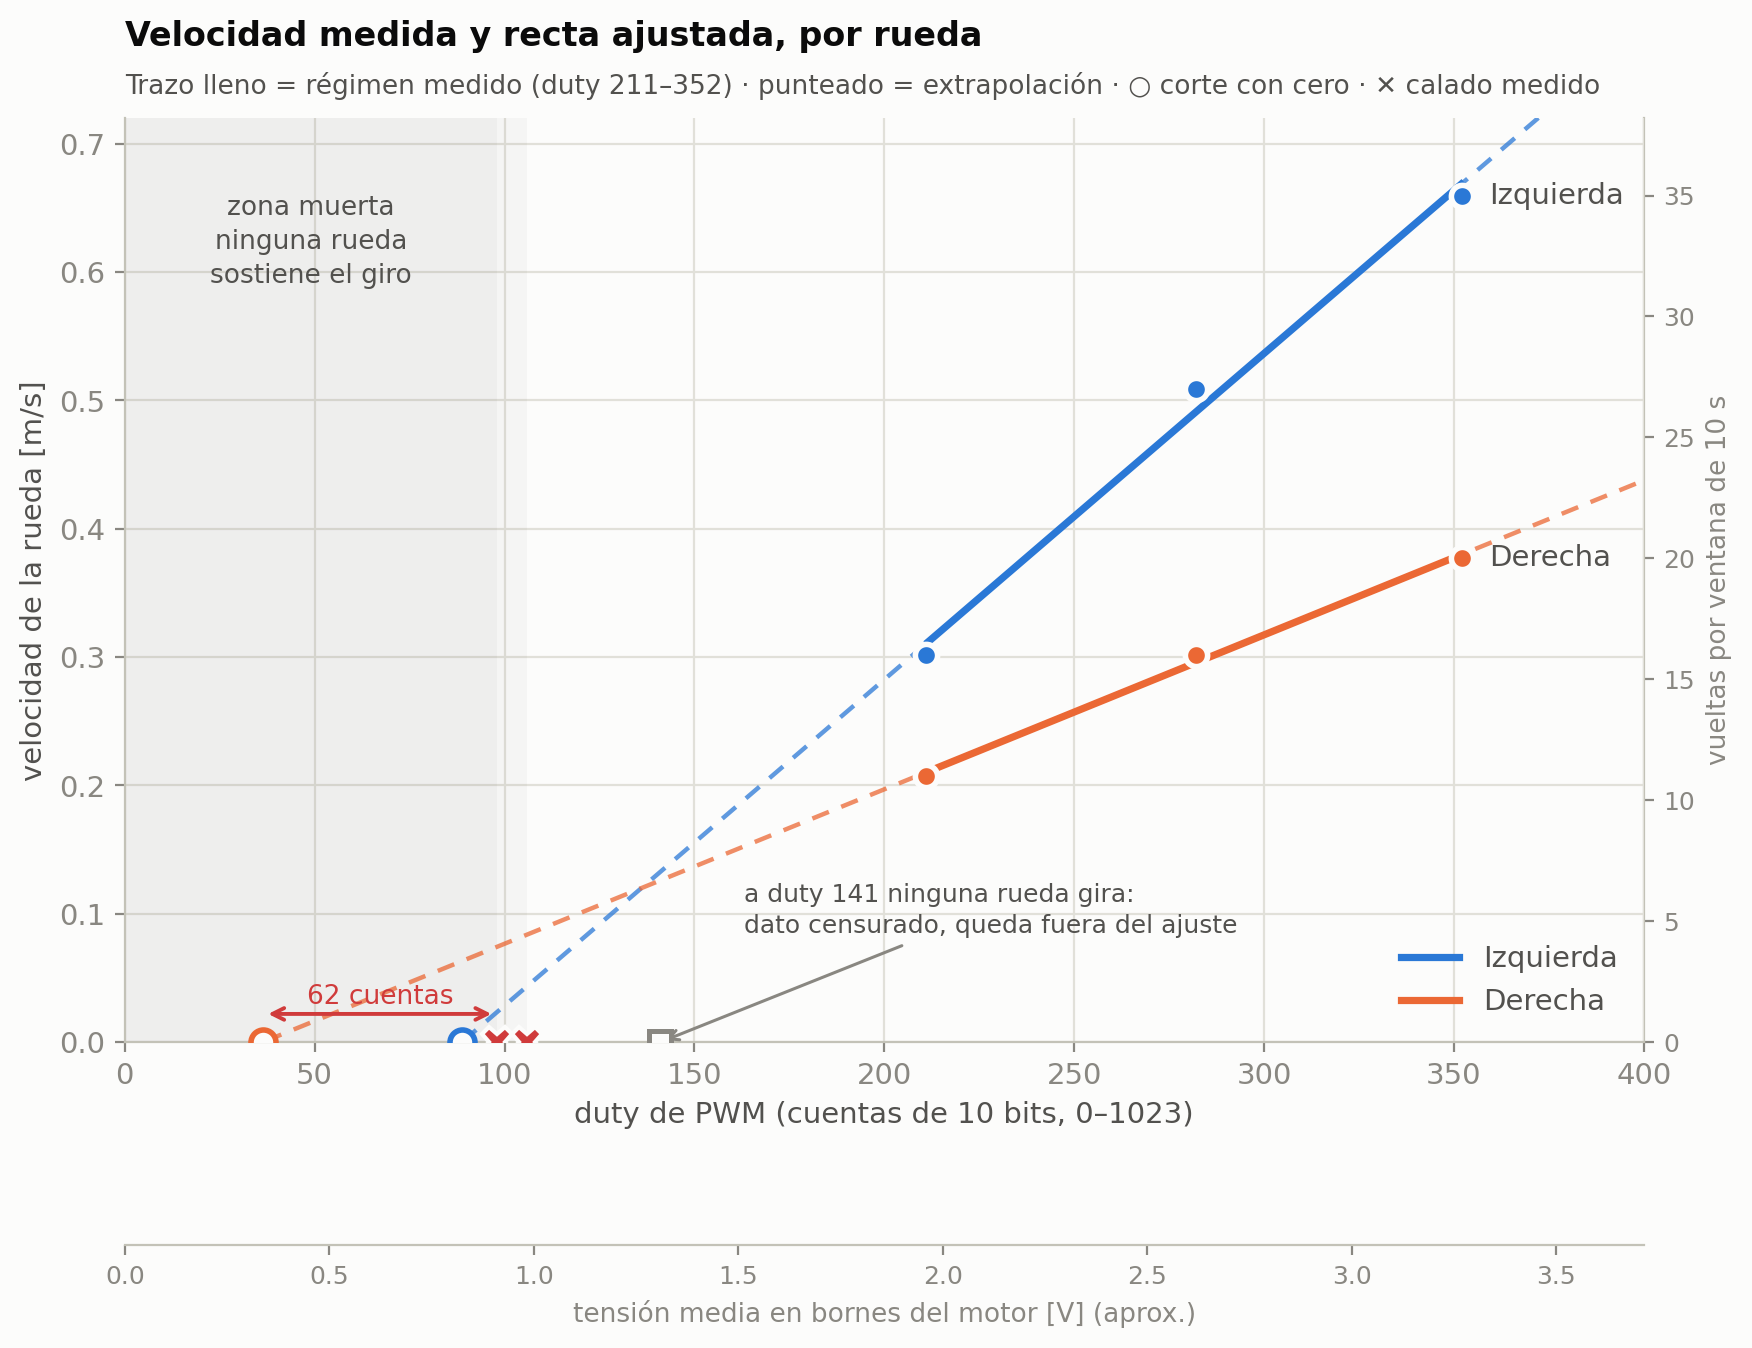
\includegraphics[height=0.64\textheight]{fig1_rectas_calibracion.png}

  \vspace{0.2em}
  \begin{columns}[T,onlytextwidth]
    \begin{column}{0.48\textwidth}
      \scriptsize
      \textbf{Lo que se esperaba:} dos motores iguales con distinta fricción, o
      sea rectas paralelas con distinto arranque.
    \end{column}
    \begin{column}{0.48\textwidth}
      \scriptsize
      \textbf{Lo que se midió:} pendientes distintas. La izquierda da
      \textbf{2,11$\times$ más velocidad por cuenta de duty}. No es fricción:
      son reducciones distintas.
    \end{column}
  \end{columns}
\end{frame}

\begin{frame}{El error que la medición destapó}
  \centering
  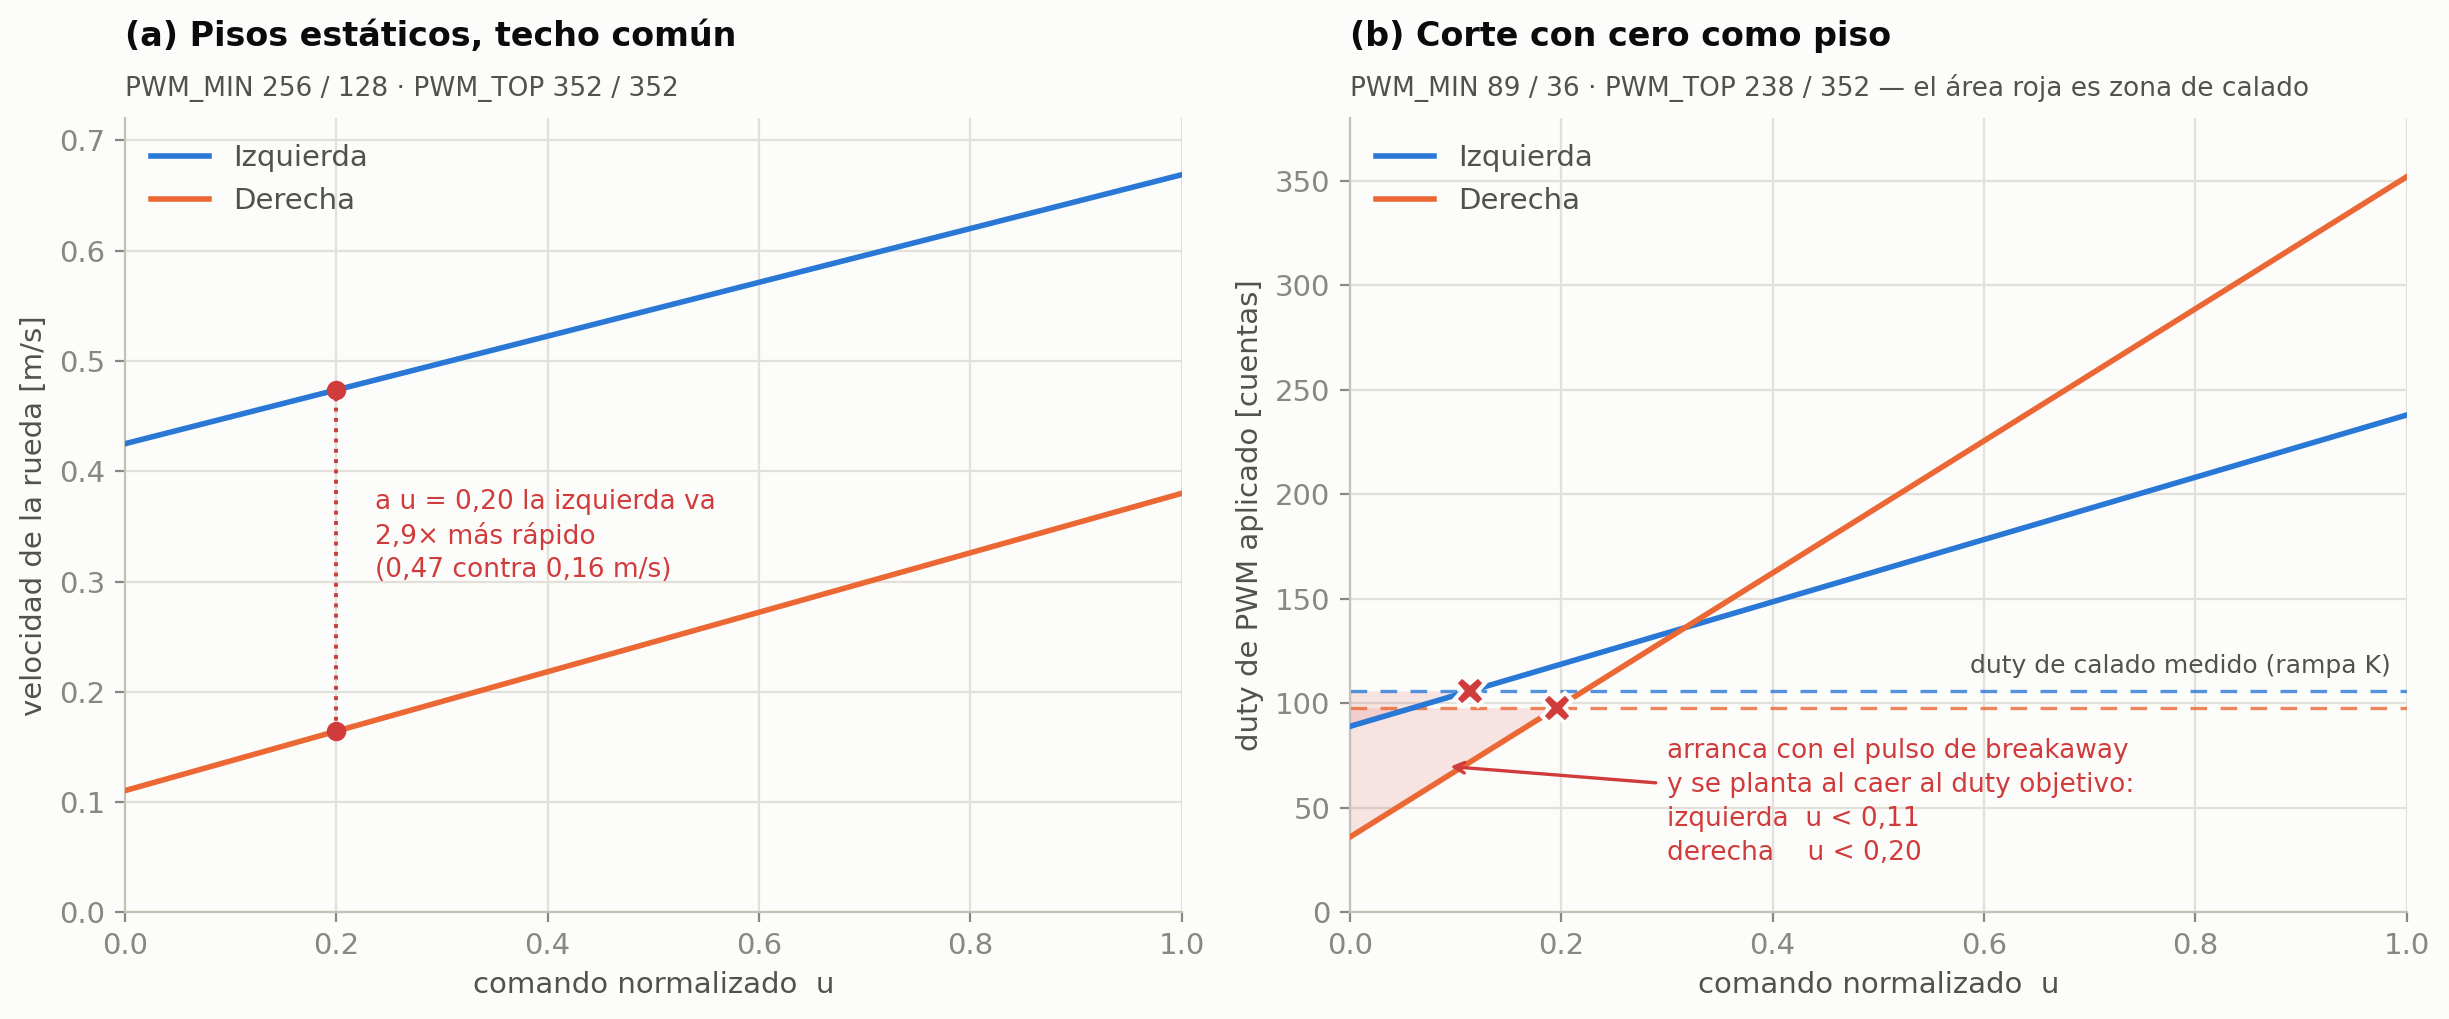
\includegraphics[height=0.52\textheight]{fig2_mapas_fallidos.png}

  \vspace{0.3em}
  \footnotesize
  \textbf{(a)} Con los umbrales estáticos, a comando 0,20 una rueda iba
  2,9$\times$ más rápido que la otra. \quad
  \textbf{(b)} Al corregirlo usando el \emph{corte con cero} de la recta como
  piso, la rueda derecha quedaba \ojo{por debajo de su duty de calado} en toda la
  parte baja del rango: arrancaba con el pulso y se plantaba.
\end{frame}

\begin{frame}{La lección metodológica --- cuatro veces el mismo error}
  \scriptsize
  \begin{table}
    \begin{tabular}{@{}p{3.2cm}p{2.9cm}p{2.6cm}p{4.0cm}@{}}
      \toprule
      \textbf{Estimación} & \textbf{Se predijo} & \textbf{Se midió} & \textbf{Dónde estaba la extrapolación} \\
      \midrule
      Caída del L298 & 1,4 V & \textbf{2,5 V} &
        Tabla del datasheet, tomada a otra corriente y temperatura \\
      Simetría de los motores & iguales, distinta fricción & \textbf{2,11$\times$ en pendiente} &
        Se supuso desde la chapa, sin medir \\
      Piso de la recta & 89 / 36 & \textbf{$\sim$106 / $\sim$98} &
        Recta ajustada entre duty 211 y 352, usada en duty $\approx$ 0 \\
      Techo de velocidad & $v_{max} = 0{,}34$ & \textbf{72} &
        Fórmula válida para el mapa anterior, aplicada al nuevo \\
      \bottomrule
    \end{tabular}
  \end{table}

  \vspace{0.4em}
  \begin{alertblock}{El tercero es el más instructivo, porque el modelo era correcto}
    \small
    $R^2 > 0{,}99$ en el régimen medido. \textbf{Lo que falló no fue el ajuste
    sino su dominio de validez}: cerca de velocidad cero la fricción crece más
    que lineal, así que la recta describe muy bien lo que se midió y \emph{no
    dice nada} sobre dónde se planta la rueda. El único remedio fue ir a medir
    ahí.
  \end{alertblock}
\end{frame}

\begin{frame}{El resultado: un rango útil que entra en el presupuesto}
  \centering
  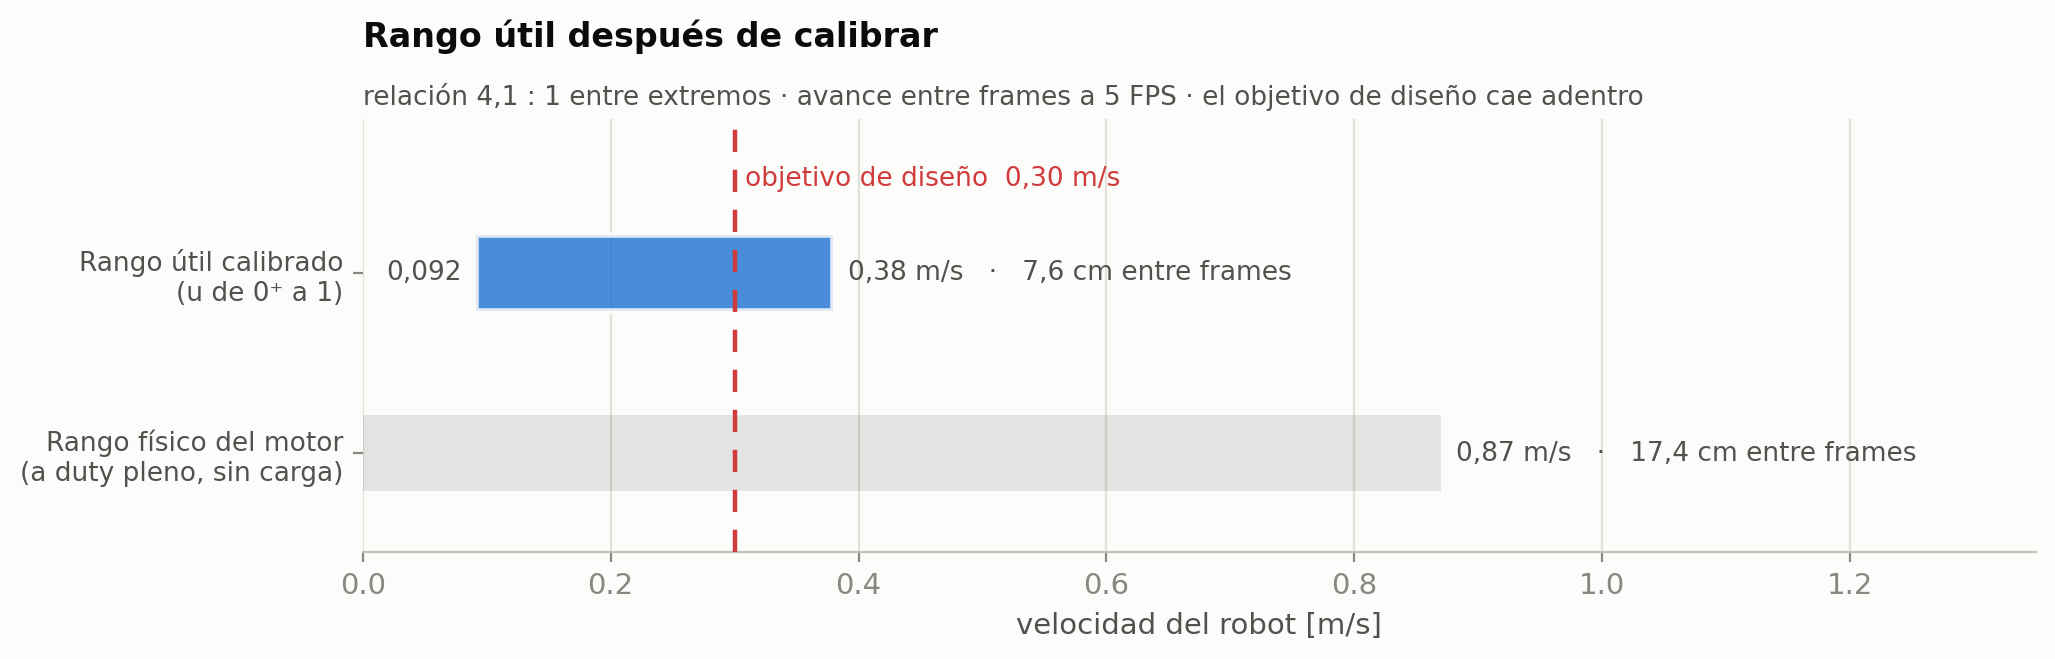
\includegraphics[height=0.46\textheight]{fig4_rango_util.png}

  \vspace{0.5em}
  \begin{columns}[T,onlytextwidth]
    \begin{column}{0.48\textwidth}
      \footnotesize
      La velocidad quedó acotada a un rango \textbf{4,1 : 1} que el lazo de visión
      puede seguir: entre 1,8 y 7,6 cm de avance entre frame y frame a 5 FPS.
    \end{column}
    \begin{column}{0.48\textwidth}
      \footnotesize
      Sin limitar, el robot iría a 0,87 m/s: \textbf{17 cm entre frames}, o sea
      controlando a ciegas la mayor parte del tiempo.
    \end{column}
  \end{columns}
\end{frame}

% =============================================================================
\section{Estado y plan}
% =============================================================================

\begin{frame}{Tablero de estado, bloque por bloque}
  \small
  \begin{columns}[T,onlytextwidth]
    \begin{column}{0.48\textwidth}
      \begin{block}{\textcolor{azul}{Raspberry Pi --- alto nivel}}
        \begin{tabular}{@{}p{0.4cm}p{4.6cm}@{}}
          \curso & Cámara Arducam (disponible) \\
          \curso & Detector YOLOv8n (código listo) \\
          \listo & Confirmación temporal \\
          \pend & Máquina de estados \\
          \pend & Ley de control \\
        \end{tabular}
      \end{block}
      \begin{block}{\textcolor{verde!60!black}{Energía}}
        \begin{tabular}{@{}p{0.4cm}p{4.6cm}@{}}
          \listo & Riel de 12 V a motores \\
          \pend & Riel de 5 V para el Pi \\
        \end{tabular}
      \end{block}
    \end{column}
    \begin{column}{0.48\textwidth}
      \begin{block}{\textcolor{naranja}{ESP32 --- bajo nivel}}
        \begin{tabular}{@{}p{0.4cm}p{4.6cm}@{}}
          \listo & Protocolo y parser \\
          \listo & Watchdog de 500 ms \\
          \listo & Mezcla diferencial \\
          \listo & Compensación de zona muerta \\
          \listo & Generación de PWM \\
          \curso & Lectura del ultrasónico (sin cablear) \\
          \curso & Buzzer (sin cablear) \\
        \end{tabular}
      \end{block}
      \begin{block}{\textcolor{gris}{Planta}}
        \begin{tabular}{@{}p{0.4cm}p{4.6cm}@{}}
          \listo & L298N y motores, calibrados \\
          \pend & Prueba de recta en piso \\
        \end{tabular}
      \end{block}
    \end{column}
  \end{columns}
\end{frame}

\begin{frame}{Qué falta, y de qué depende cada cosa}
  \centering
  \resizebox{\textwidth}{!}{%
  \begin{tikzpicture}[font=\scriptsize,
      p/.style={draw, rounded corners=3pt, minimum height=1.15cm, text width=2.7cm,
                align=center, line width=0.8pt},
      f/.style={-{Stealth[length=2mm]}, line width=0.8pt}]
    \node[p, draw=ambar, fill=ambar!10] (d3) {\textbf{Día 3}\\ Medir el FPS\\ en el Pi};
    \node[p, draw=gris, fill=gris!8, below=0.7cm of d3] (rec) {\textbf{Prueba de recta}\\ desvío en 2 m};
    \node[p, draw=gris, fill=gris!8, below=0.7cm of rec] (ult) {\textbf{Cablear}\\ ultrasónico y buzzer};

    \node[p, draw=azul, fill=azul!10, right=1.9cm of d3] (d4) {\textbf{Día 4}\\ Estados + control\\ (ruedas al aire)};
    \node[p, draw=azul, fill=azul!10, right=1.9cm of d4] (d5) {\textbf{Día 5}\\ Calibrar en piso\\ $K_p$, área, tiempos};
    \node[p, draw=verde!60!black, fill=verde!10, right=1.9cm of d5] (d7) {\textbf{Días 6--7}\\ Métricas, demo\\ e informe};

    \draw[f] (d3) -- node[above,font=\tiny,align=center]{fija el\\presupuesto} (d4);
    \draw[f] (ult.east) -- node[below,pos=0.6,font=\tiny,align=center]{habilita el criterio\\duro de llegada} (d4.south west);
    \draw[f] (rec.east) -- node[above,pos=0.6,font=\tiny,align=center]{decide si\\hacen falta encoders} (d4.west);
    \draw[f] (d4) -- (d5);
    \draw[f] (d5) -- (d7);
  \end{tikzpicture}}

  \vspace{0.6em}
  \begin{block}{Los tres pendientes de la izquierda son independientes entre sí}
    \small
    El \textbf{Día 3} sólo necesita el Pi y la cámara; los otros dos, el robot.
    Se pueden hacer en cualquier orden --- pero el Día 3 es el que más destraba,
    porque el FPS medido es lo que fija el presupuesto de todo el lazo de control.
  \end{block}
\end{frame}

\begin{frame}{Riesgos vivos y cómo están mitigados}
  \scriptsize
  \begin{table}
    \begin{tabular}{@{}p{4.3cm}p{1.6cm}p{6.3cm}@{}}
      \toprule
      \textbf{Riesgo} & \textbf{Prob.} & \textbf{Mitigación} \\
      \midrule
      FPS insuficiente en el Pi & Media &
        Bajar a 320$\times$320, exportar a NCNN, procesar 1 de cada 2 frames.
        \emph{El banco de medición ya dice cuál corresponde.} \\
      El Pi se reinicia al arrancar los motores & \textbf{Alta} &
        Alimentación separada desde el día 1. No es opcional. \\
      Detección inestable a distancia & Media &
        Acercar el escenario, bajar el umbral de confianza, objetos más grandes. \\
      El robot oscila al aproximarse & Media &
        Reducir $K_{p,ang}$ y agregar zona muerta alrededor del centro.
        \emph{Sabemos que hace falta: el escalón de arranque lo garantiza.} \\
      La marcha recta se curva & \textbf{Confirmada} &
        Calibración por rueda (hecha). Si no alcanza, encoders. \emph{La prueba
        de recta es la que decide.} \\
      Falla total de la detección & Baja &
        \emph{Fallback:} marcadores ArUco. Sólo si todo lo demás falla, porque
        reduce el componente de IA. \\
      \bottomrule
    \end{tabular}
  \end{table}
\end{frame}

\begin{frame}{Cómo se va a evaluar}
  \scriptsize
  \begin{table}
    \begin{tabular}{@{}p{5.0cm}p{5.2cm}p{2.2cm}@{}}
      \toprule
      \textbf{Métrica} & \textbf{Cómo se mide} & \textbf{Objetivo} \\
      \midrule
      FPS de inferencia & Promedio del lazo en el Pi & $\geq$ 5 \\
      Tasa de detección & \% de frames con el objeto presente donde fue detectado & $\geq$ 80 \% a 2 m \\
      Falsos positivos & Detecciones espurias por minuto, sala vacía & $<$ 1/min \\
      Éxito de aproximación & Corridas que terminan en ENCONTRADO sin chocar & $\geq$ 8/10 \\
      Éxito de escape & Corridas que completan la maniobra sin chocar & $\geq$ 8/10 \\
      \textbf{Arbitraje de conflicto} & Corridas con ambos objetos donde prioriza huir & \textbf{10/10} \\
      Tiempo hasta encontrar & Desde el inicio hasta ENCONTRADO, objeto a 2 m & registrar \\
      Latencia de reacción & Desde que aparece la mochila hasta que arranca la huida & registrar \\
      \bottomrule
    \end{tabular}
  \end{table}

  \vspace{0.4em}
  {\centering\small
    Los criterios están definidos \textbf{antes} de las pruebas. Definirlos
    después es ajustar la vara al resultado.\par}
\end{frame}

% =============================================================================
\begin{frame}[standout]
  Resumen en tres frases
\end{frame}

\begin{frame}{Para llevarse}
  \begin{enumerate}
    \item \destaca{La arquitectura es de dos niveles y esa es la decisión que
          ordena todo lo demás.} El Pi decide qué hacer a 5--15 Hz y sin
          garantías; el ESP32 ejecuta a 100 Hz con garantías. Ninguna función
          crítica depende de código complejo.

    \vspace{0.4em}
    \item \destaca{El lazo de control se cierra por el mundo físico.} No hay
          sensor que mida ``estoy apuntando al objetivo'': lo mide el frame
          siguiente. Por eso el FPS de la cámara \emph{es} la frecuencia del
          lazo, y por eso medirlo es el próximo paso.

    \vspace{0.4em}
    \item \destaca{La mitad del trabajo real estuvo en la planta, no en la IA.}
          Cuatro estimaciones razonables cayeron por medición, todas por el mismo
          motivo: extrapolar un modelo fuera del rango donde se lo validó. Es el
          hilo conductor del informe.
  \end{enumerate}

  \vspace{0.8em}
  {\centering\small
    \textbf{Próximo paso concreto:} correr el banco de visión en el Pi y anotar
    el FPS.\par}
\end{frame}

\end{document}
